\section{Pressure Vessels}

\subsection{\blue{Thin-Walled Pressure Vessels}}
\begin{itemize}
    \item Inner radius: $r$
    \item Wall thickness: $t$
    \item Thin walls: $t/r << 1$
    \item Assume that stress distribution through the thin wall is uniform
    \item Pressure vessel contains fluid under pressure p (understood to be gauge pressure, i.e., $p = \Delta p = p_i - p_o$)
\end{itemize}

\subsubsection{\blue{Cylindrical Vessels}}

\begin{figure*}[!h]
\centering
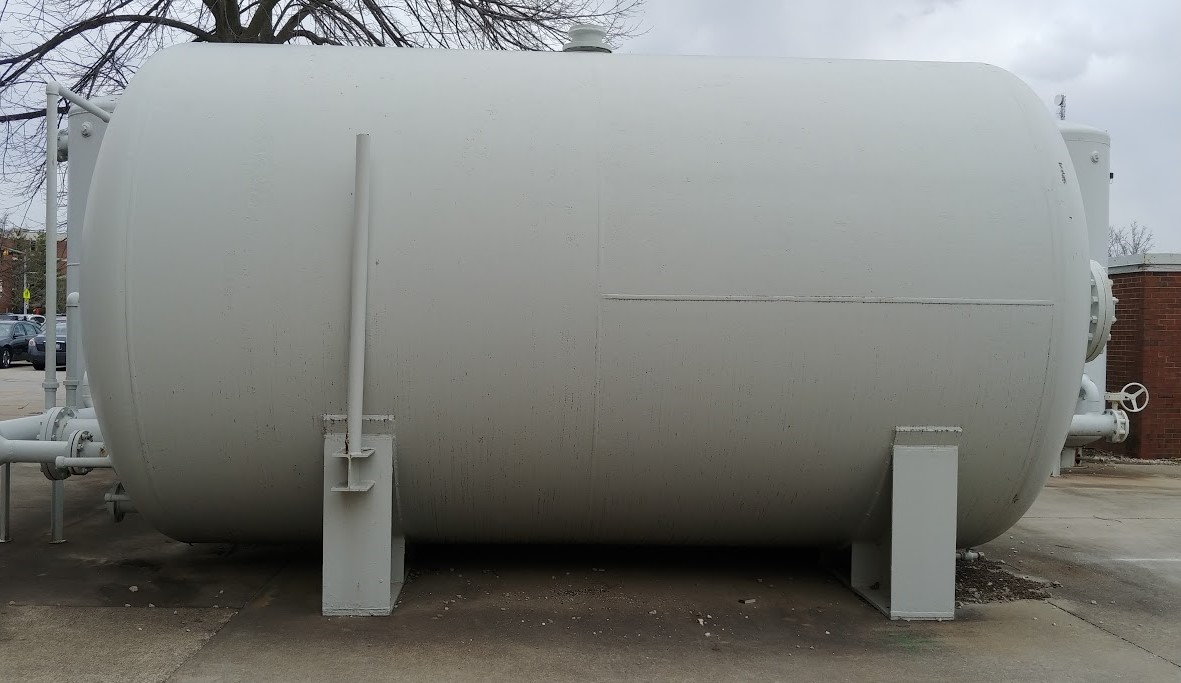
\includegraphics[angle=0, width=3in]{Pressure Vessels-Figures/cylindrical_vessel_example.jpg}
\vspace{-2mm}
\caption{\small Cylindrical pressure vessel behind Transportation Building.}
\vspace{-3mm}
\label{Fig:CylindricalVesselEx}
\end{figure*}

\noindent Cylindrical pressure vessels are an axisymmetric problem, there is no shear stress on an element parallel to the axis of the cylinder. Therefore, the only normal stresses are in the directions of axis and circumference.

\begin{figure*}[!h]
\centering
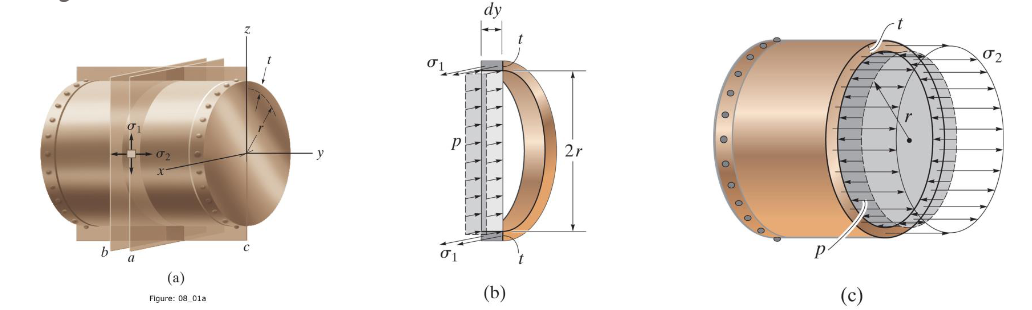
\includegraphics[angle=0, width=6in]{Pressure Vessels-Figures/CylindricalVessel.png}
\vspace{-2mm}
\caption{\small \blue{Taken from TAM251 Lecture Notes - L8S4}}
\vspace{-3mm}
\label{Fig:CylindricalVessel}
\end{figure*}

\noindent \textbf{Hoop stress:} (circumferential stress): \[\sigma_1 = \sigma_h = \frac{pr}{t}\]

\noindent \textbf{**Expandable Derivation**}
\[\sum F_z: \sigma_h (2t \Delta x) - p(2r \Delta x)=0\]
\[\therefore \sigma_h = \frac{pr}{t}\]
\noindent \textbf{**End Derivation**}

\noindent \textbf{Axial stress:} (longitudinal stress): \[\sigma_2 = \sigma_a = \frac{pr}{2t}\]

\noindent \textbf{**Expandable Derivation**}

\noindent The force of the fluid in the longitudinal direction will be the internal pressure, $p$, times the area of the fluid within the vessel, $\pi r^2$. Similarly, the force within the vessel wall in the longitudinal direction will be the stress, $\sigma_a$, times the area of the wall. We assume we can unravel the thin wall of the pressure vessel, simplifying the area of the thin wall as the circumference, $2\pi r$, multiplied by the thickness, $t$.

\[\sum F: \sigma_a (2\pi r t) - p(\pi r^2)=0\]
\[\therefore \sigma_a = \frac{pr}{2t}\]

\noindent \textit{Note:} A more accurate derivation of the longitudinal stress may be calculated with the true area of the pressure vessel $(A_{wall} = \pi(r+t)^2 - \pi r^2 = \pi 2rt + \pi t^2)$, leading to an axial stress of: $\sigma_a = \frac{pr^2}{2rt + t^2}$. The approximation used in this course is only sufficient when $\frac{r}{t} \ge 10$. 

\vspace{5pt}

\noindent \textbf{**End Derivation**}

\vspace{5pt}

\noindent \textbf{Radial Stress:}

\begin{figure*}[!h]
\centering
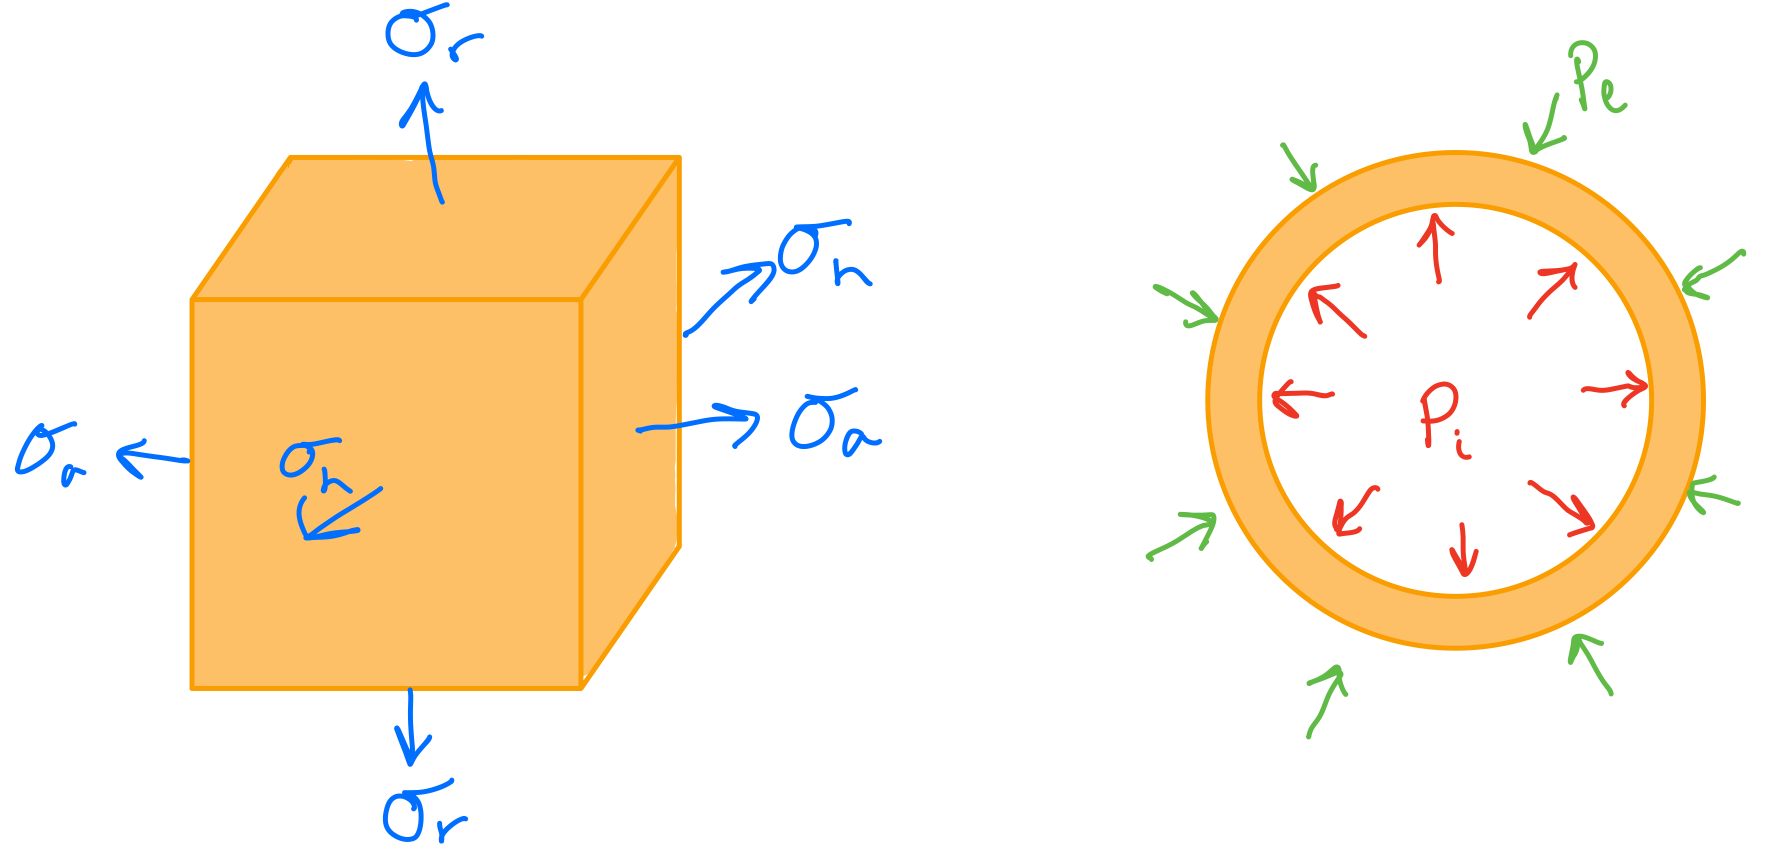
\includegraphics[angle=0, width=4in]{Pressure Vessels-Figures/RadialStress.png}
\vspace{-2mm}
\caption{\small \blue{Taken from TAM251 Lecture Notes - L8S5}}
\vspace{-3mm}
\label{Fig:RadialStress}
\end{figure*}

\begin{itemize}
    \item Inner Surface: $\sigma_r = -p$
    \item Outer Surface: $\sigma_r = 0$
\end{itemize}

\noindent Because $t/r << 1$: \[\sigma_h,\sigma_a >> \sigma_r\] so in general we can \textit{neglect $\sigma_r$}

\subsubsection{\blue{Spherical Vessels}}

\begin{figure*}[!h]
\centering
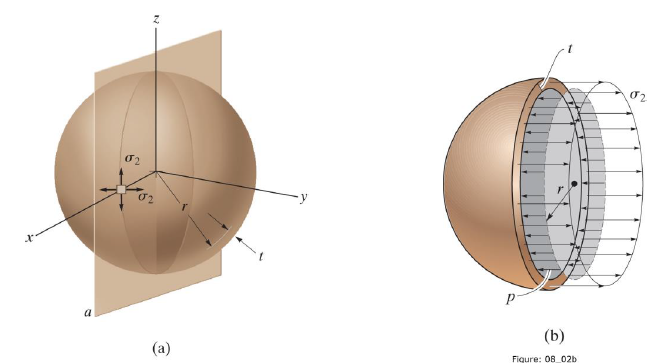
\includegraphics[angle=0, width=4in]{Pressure Vessels-Figures/SphericalVessel.png}
\vspace{-2mm}
\caption{\small \blue{Taken from TAM251 Lecture Notes - L8S6}}
\vspace{-3mm}
\label{Fig:SphericalVessel}
\end{figure*}

\noindent Due to symmetry: \[\sigma_1 = \sigma_2 = \frac{pr}{2t}\]